% Drawing 154/07-23 -- folder 154, batch 07, archive page 132 (PDF page 133).
% Transcription: à côté, un petit dessin : un croisement orange sur la droite vert clair $D$, orientée par $\omega$ (flèche), le sommet $s$ et, au-dessous, la rive brune $\rho$
% Kind: crossing on the line D with its bank rho. Method 2 (schematic redraw from the facsimile). Status: ok.
% Notes: Two orange strokes crossing on the light green line (point computed), the line ending in an arrowhead with D written after it, s beside the crossing, a short brown stroke under the line on the left with rho below it, and the small arrow omega under the line. Redrawn 2026-11-12 (issue 128): to check again.
% Coordinates: 1 unit = 1 mm = 1/100 of the crop width (bbox in page fractions: [0.715, 0.335, 0.885, 0.395]).
% Redrawn by Claude (claude-fable-5-2), issue #128, 2026-11-12; not checked by a human; not compiled (no TeX in the session).
% Rights: reproduces part of the work -- behind RENDER_TRANSCRIPTS, never published by itself.
\documentclass[tikz,border=3pt]{standalone}
\usepackage{amsmath,amssymb}
\usetikzlibrary{patterns,arrows.meta}
\tikzset{Or/.style={orange!90!black}, Lg/.style={green!60!black!70}, Br/.style={brown!80!black}, pencil/.style={black!45}, struck/.style={black!35}, mpt/.style={circle,draw,inner sep=1.3pt}, pt/.style={circle,fill,inner sep=0.9pt}, opt/.style={circle,draw,fill=white,inner sep=1.1pt}}
\begin{document}
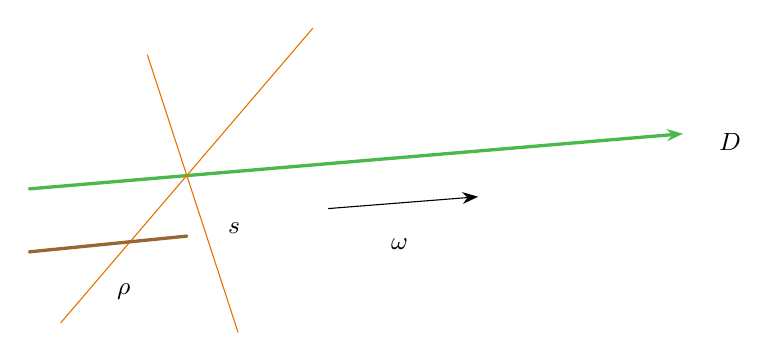
\begin{tikzpicture}[x=1mm,y=1mm,line cap=round,line join=round,font=\scriptsize]
\draw[Lg,very thick,-{Stealth[length=2mm]}] (5,-54) -- (88,-47);
\draw[Or] (9,-71) -- (41,-33.6);
\draw[Or] (20,-37) -- (31.5,-72.2);
\draw[Br,very thick] (5,-62) -- (25,-60);
\node[inner sep=1pt] at (94,-48) {\small $D$};
\node[inner sep=1pt] at (31,-59) {\small $s$};
\node[inner sep=1pt] at (17,-67) {\small $\rho$};
\draw[-{Stealth[length=2mm]}] (43,-56.5) -- (62,-55);
\node[inner sep=1pt] at (52,-61) {\small $\omega$};
\end{tikzpicture}
\end{document}
